\documentclass[11pt,xcolor=svgnames]{beamer}
\usepackage{dsfont,natbib,setspace,changepage,multirow}
\mode<presentation>

% replaces beamer foot with simple page number
\setbeamertemplate{navigation symbols}{}
\setbeamercolor{frametitle}{fg=black}
\setbeamerfont{frametitle}{series=\bfseries}
\setbeamerfont{frametitle}{size=\normalsize}

\setbeamercolor{frametitle}{fg=black}
\newcommand{\theme}{\color{Maroon}}

\setbeamertemplate{footline}{
   \raisebox{5pt}{\makebox[\paperwidth]{\hfill\makebox[20pt]{\color{gray}\scriptsize\insertframenumber}}}}

\usepackage{tikz}

\graphicspath{{../graphs/}}

\setbeamercolor{whitebox}{bg=gray!10}

% colors
\newcommand{\bk}{\color{black}}
\newcommand{\rd}{\color{red}}
\newcommand{\fg}{\color{ForestGreen}}
\newcommand{\bl}{\color{blue}}
\newcommand{\gr}{\color{black!60}}
\newcommand{\sg}{\color{DarkSlateGray}}
\newcommand{\br}{\color{SaddleBrown}}
\newcommand{\nv}{\color{Navy}}


% common math markups
\newcommand{\bs}[1]{\boldsymbol{#1}}
\newcommand{\mc}[1]{\mathcal{#1}}
\newcommand{\mr}[1]{\mathrm{#1}}
\newcommand{\bm}[1]{\mathbf{#1}}
\newcommand{\ds}[1]{\mathds{#1}}
\newcommand{\indep}{\perp\!\!\!\perp}

% spacing and style shorthand
\setstretch{1.1}

% shorthand
\newcommand{\sk}{\vspace{.5cm}}
\newcommand{\R}[1]{{\tt \nv #1}}
\newcommand{\til}{{\footnotesize$\bs{\stackrel{\sim}{}}$}}
\DeclareSymbolFont{extraup}{U}{zavm}{m}{n}
\DeclareMathSymbol{\vardiamond}{\mathalpha}{extraup}{87}

\begin{document}

\setcounter{page}{0}
{ 
\usebackgroundtemplate{
\includegraphics[height=\paperheight]{phoenix}}
\begin{frame}[plain]
\begin{center}


{\bf \Large [4] Big Data: Treatment Effects }

\vskip 1.5cm 
Matt Taddy, University of Chicago Booth School of Business

\vskip .2cm 
\texttt{faculty.chicagobooth.edu/matt.taddy/teaching} 


\end{center}
\end{frame} }

%\setbeamercolor{background canvas}{bg=gray!10}
\begin{frame}
{[4] \theme Estimation of Treatment Effects}

Today we'll try for `real' patterns: \\~~~~those that represent some true underlying mechanism.

\vskip .5cm
First, a quick trip through the gold standard: experiments.

\vskip .5cm
Second, we look at causal inference without an experiment.

\vskip .5cm
Finally, we see a new tool for uncertainty quant: the bootstrap

\end{frame}

\begin{frame}
{Causal Inference}

We've used {\it prediction} as a basis for model building: 

\vskip .1cm
~~{\nv choose a fitting
routine to do the best job forecasting $y$ at \\~~new $\bm{x}$ drawn from the same
distribution as data sample $\bm{X}$.}

\vskip .1cm
{ This exactly the question tackled by CV and AICc. }

\vskip .5cm
Today, we'll try to estimate the effect of a special covariate:

\vskip .1cm
 {\theme ~~Treatment `$d$', which we can change {\it independently} from $\bm{x}$.}

\vskip .1cm
That is: we want to know the causal {\it treatment effect} (TE).

\vskip .25cm
{For example,
\begin{itemize}
\item $d=1$ if you get the drug, $d=0$ for placebo (control).
\item $d$ is some {\it policy tool}, like interest rates or product price.
\end{itemize}}

\end{frame}


\begin{frame}

Our treatment effect (TE) model looks like
\[
\ds{E}[y|d,\bm{x}] = \alpha + d\gamma + \bm{x}'\bs{\beta}
\]
and we'll want to interpret {\it treatment effect} $\gamma$ causally.

\vskip .5cm 
A coefficient is {\theme structural} or {\theme causal} if it is a {\it real-world} effect.

$ \Rightarrow \gamma$ must represent change in $y$ when $d$ moves {\it independent} \\~~~~of any other influencers
(both in $\bm{x}$ or those we've ommitted).

\vskip .5cm
In contrast, a {\nv reduced form} model is a simple representation for the effect of $\bm{x}$ on $y$, without 
worying about causal mechanisms.

\vskip .1cm
{\gr e.g., in reduced form, $\beta_j$ is the effect of 
$x_j$, but this could  be due to $x_j$'s correlation with  other variables that actually cause $y$.}

\end{frame}


\begin{frame}
{Randomized Control Trials: {\theme A/B experiments}}

We want to know the effect on $y$ of\\ change in $d$ independent of change in $\bm{x}$.

\vskip .5cm
A {\it completely randomized design} draws two random samples of units, then applies $d=0$ to one sample  and $d=1$ to the other.

\vskip .25cm
{\color{black!70} For example, you randomize your website visitors into groups `A' (control) and `B' (treatment).  Those in A see the current website, while those in B see a new layout.  }

\vskip .25cm
Say $y$ (spend or clicks) is the response of interest.  \\TE is treatment mean minus control mean:
$\theme
\hat \gamma = \bar y_B - \bar y_A
$

\vskip .25cm
{\gr $\mathrm{se}(\hat \gamma) = \sqrt{SST_A/n_A^2 + SST_B/n_B^2}$ and this is just stats 101.}
\end{frame}

\begin{frame}
{$\vardiamond$ RCT and Sequential Design}

RCT (A/B) experiments are hugely popular and hugely useful.

\vskip .25cm
If you have the ability to randomize, it is very tough to find a TE estimate that is much better than $\bar y_B - \bar y_A
$ from an experiment. {\gr Indeed: beware of those who claim otherwise.}

\vskip .5cm
However, it's century-old tech and sometimes we can do better.


This is especially true if:
\begin{itemize}
\item You view TE $\gamma(\bm{x})$ as a function of covariates.
\item You have many treatments to choose amongst.
\end{itemize}
In each case, if you are accumulating data over time you can use existing observations to guide where you sample next.  

\vskip .2cm
This is called {\theme active learning} (AL).

\end{frame}



\begin{frame}
{$\vardiamond$ Active Learning}

Say you have $j = 1 \ldots J$ different `ad campaigns' to show.

\vskip .05cm
As each user $i$ comes, you can show them one ad: $d_i=j$.

\vskip .05cm
Your goal is to maximize ad-clicks.

\vskip .5cm
Say $\bm{c}_n = [c_{n1} \dots c_{nJ}]$ are the clicks on each ad after $n$ users,

and $\bm{s}_n = [s_{n1} \dots s_{nJ}]$ are times each ad has been shown.

\vskip .5cm
To find the best ad as quickly as possible you can sample \\{\it click probabilities}
for each ad as $q_{nj} \sim \mr{Beta}(c_{nj}, s_{nj}-c_{nj})$.
\vskip .05cm
{\gr Beta has mean $c_{nj}/s_{nj}$ here, with variance that shrinks with $s_{nj}$}

\vskip .5cm
The result is that you try (explore) all the ads, but show the  ones that seem to be working more than the others.  

\vskip .1cm
{\theme Run \texttt{mab.R} to see this in action.}


\end{frame}

\begin{frame}
{$\vardiamond$ Bandits and more}

The prev slide's setup is called a {\nv multi-armed bandit}.

\vskip .05cm
The learning algorithm is called {\nv thompson sampling}.

\vskip .25cm
Active learning is a big area.  It gets tricky once covariates are involved {\gr (e.g., click probs are functions of user attributes.) }

\vskip .25cm
With the trend of {\it site personalization}, more and more datasets for online behaviour are coming from some AL scheme.

\vskip .5cm
AL is just one example of how the data you'll have to analyze can be much more complex than that from an A/B experiment.  

\vskip .1cm
~~{\theme In many cases, you don't get to experiment at all!}


\vskip .1cm
To figure out causal effects in more complex setups, we need to go back in time and take a look at some linear models.



\end{frame}

{\usebackgroundtemplate{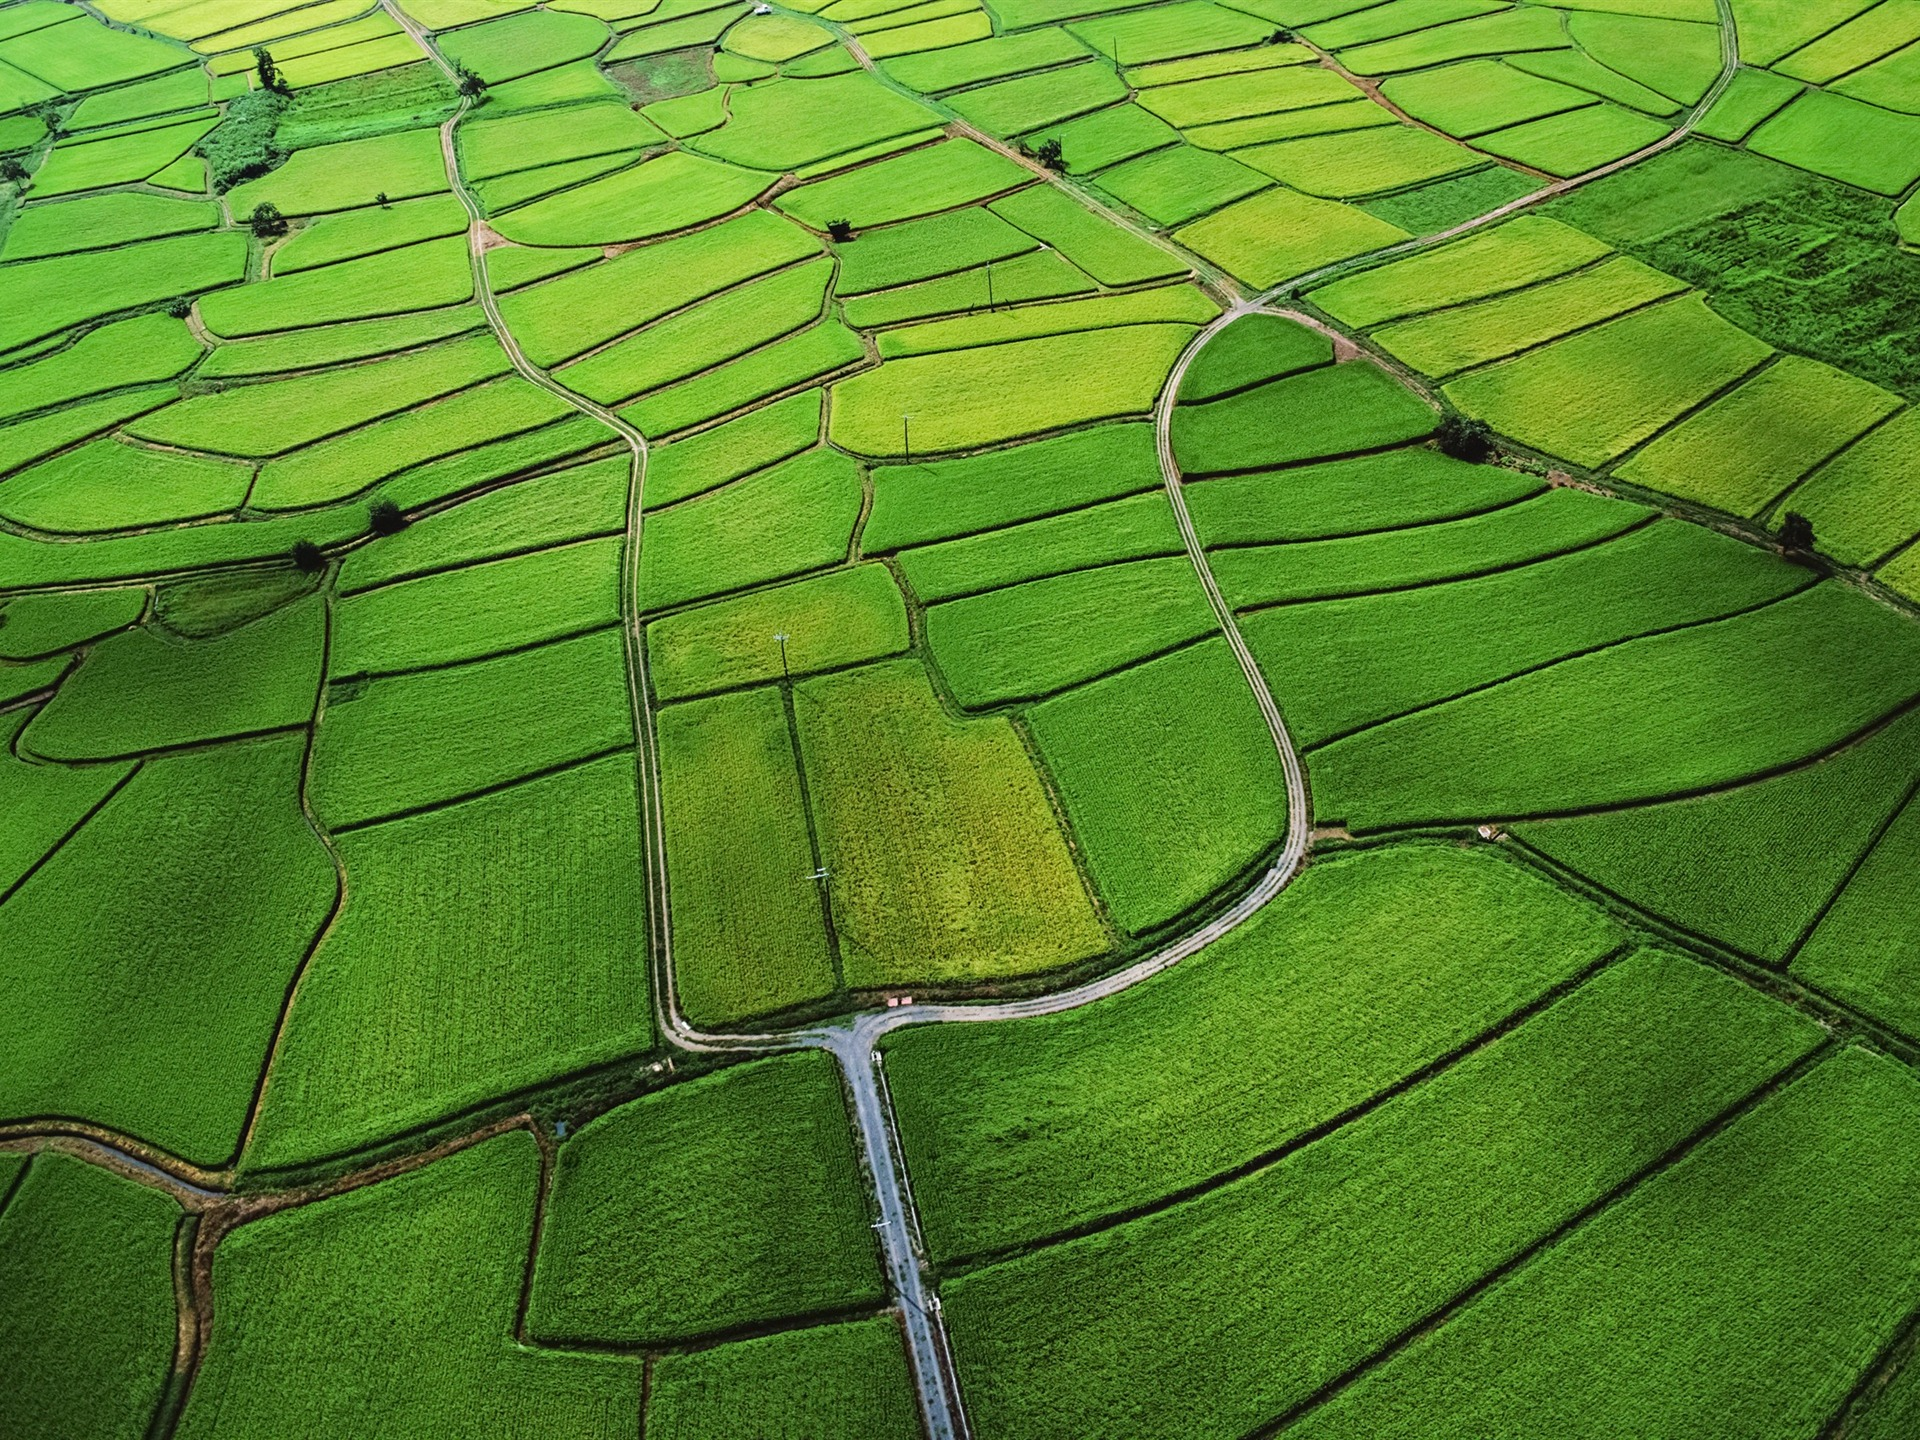
\includegraphics[height=\paperheight]{rice_fields}}
\begin{frame}{\bf \color{white} Blocked-Design Experiment}
\sk
\begin{beamercolorbox}[sep=2mm,wd=3.95in]{whitebox}
Ideas born in agriculture: ``does this fertilizer work?''

TE can get swamped by variation in growing conditions.
\end{beamercolorbox}


\vskip .25cm
\begin{center}
\begin{beamercolorbox}[sep=2mm]{whitebox}\small
Pick {\it blocks} of nearby fields and split them.

\vskip .2cm
1:~\begin{tabular}{|c|c|}
\hline
$d=0$ & $d=1$\\ 
\hline
\end{tabular}~
2:~\begin{tabular}{|c|}
\hline
$d=0$ \\ \hline $d=1$\\ 
\hline
\end{tabular}
~
3:~\begin{tabular}{|c|c|}
\hline
$d=1$ & $d=0$\\ 
\hline
\end{tabular}~
4:~\begin{tabular}{|c|}
\hline
$d=1$ \\ \hline $d=0$\\ 
\hline
\end{tabular}

\vskip .2cm Response $y_{kd}$ is some measure of yield (e.g., kg of rice).
\end{beamercolorbox}
\end{center}

\sk\sk\sk
\hfill\begin{beamercolorbox}[sep=2mm,wd=3.9in]{whitebox}
The estimated {\it treatment effect} is $\hat \gamma = \frac{1}{4}\sum_{k=1}^4(y_{k1} - y_{k0})$
\end{beamercolorbox}

\end{frame}}

\begin{frame}
{Blocked-Design Experiment}

Re-write the TE model as a regression
\[
\ds{E}[y|d,k] = \alpha_k + d\gamma 
\]
where $\alpha_k$ is the intercept for block $k$.
\vskip .1cm
$\hat \gamma$ for this regression is $\frac{1}{4}\sum_{k=1}^4(y_{k1} - y_{k0})$,  as on prev slide.


\vskip .5cm
Here, we interpret $\gamma$ as a {\it causal effect}
{\gr (not just correlation)}\\ because   treatment $d=0/1$ is independent of the covariates.
{\gr (in this case, `covariates' = block membership factor variables).}

\vskip .1cm
We know this because that's how the experiment was designed.

\vskip .5cm
{\theme Big lesson: we can use regression to analyze experiments!}

\end{frame}

\begin{frame}
{SEM Experiment example}

\vskip .25cm
What is the effect of {\it paid search advertising?}

{\gr Or, if we turned it off and went organic, what would happen?}

\vskip .5cm
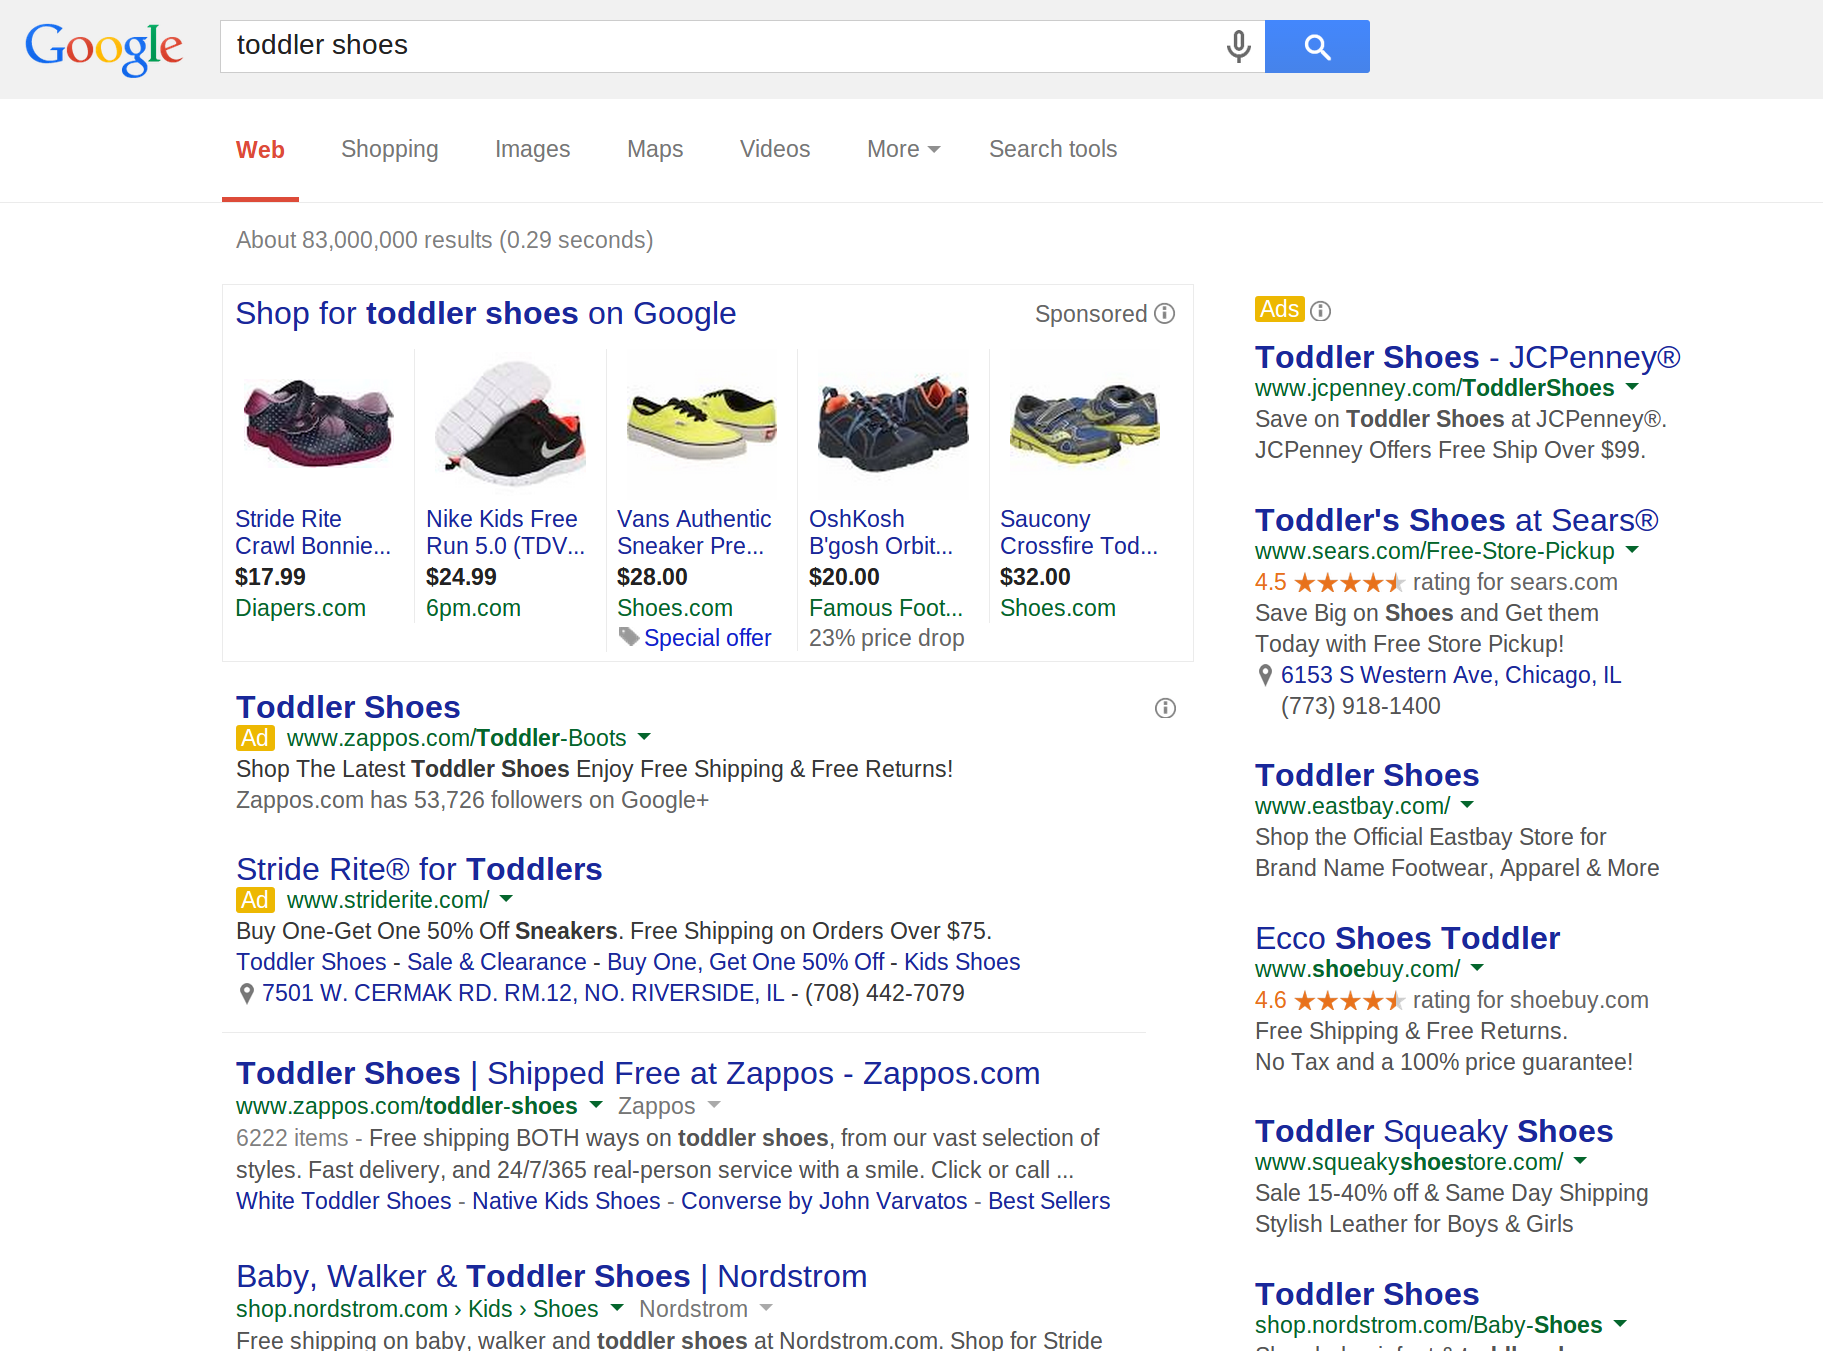
\includegraphics[width=4.25in]{toddlershoes}
\end{frame}

\begin{frame}
{Correcting for {\theme incomplete} randomization}

eBay did a big experiment to test paid search (aka, SEM)

{\gr Blake + Nosko + Tadelis: Paid Search Effectiveness.}

\sk
They {\it turned off} paid search (stopped bidding on any AdWords) for 65 of the 210
`Designated Market Areas' (DMA) in the US.  \\ {\gr (Google guesses the DMA for a browser.)}

\sk
In 2012, eBay recorded revenue in all DMAs for $\approx 8$ weeks before and after turning off SEM for the treated 65 on May 22.

\sk
Data are in {\tt paidsearch.csv}, and code is  {\tt paidsearch.R}.
{\gr Note that this is not the real data; it's been scaled and shifted.}
\end{frame}

\begin{frame}

Problem: the treated DMAs are not a random sample.  \\They avoided, e.g., the largest markets.



\begin{center}
{\it \footnotesize Avg Revenue; dashed line is May 22, when SEM turns off for treated} 
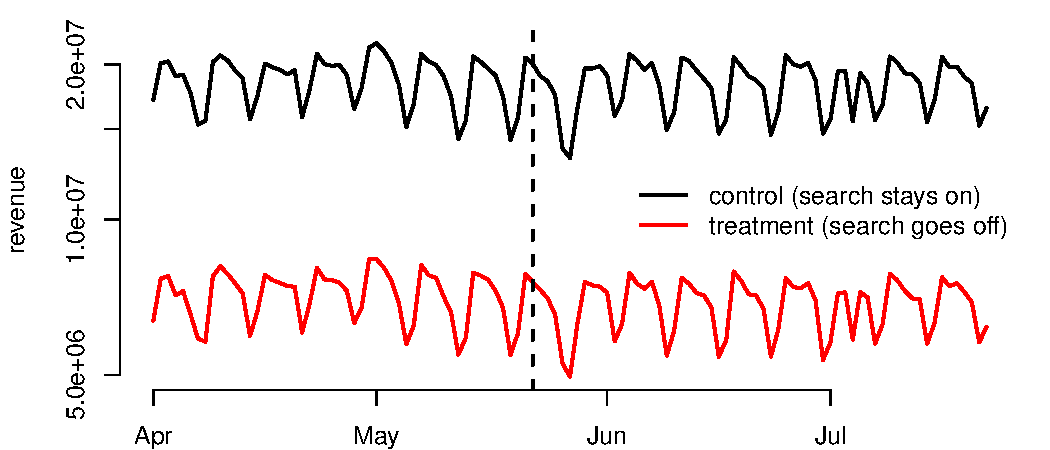
\includegraphics[width=4in]{SEMrev}
\end{center}



If you just look at $\bar y_B - \bar y_A$, you see a big difference even before SEM turns off (i.e., before B is {\it treated}).  This can't be causal!

\end{frame}

\begin{frame}


If SEM works, then the revenue difference should be {\it larger after search is turned of for treatment DMAs}  (after May 22).
{\gr We'll look at differences in log(revenue).}

\begin{center}
{\footnotesize \it log(avg control revenue) - log(avg treatment revenue)}
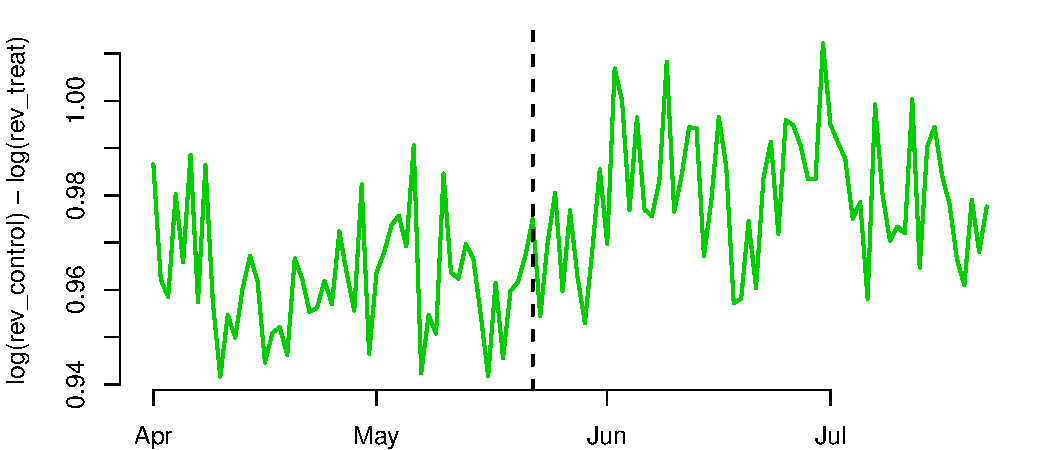
\includegraphics[width=4in]{SEMdiff}
\end{center}


{{\it Maybe} there is some increase. Is it real?}

\end{frame}


\begin{frame}

{\gr This is a more complicated blocking structure than before.

But we can still write out a similar regression model.}

\vskip .5cm
Say you have DMA $i$ at time $t \in {0,1}$, before or after May 22,
and $d_i = 1$ if DMA $i$ is in treatment group, 0 otherwise.

Response  $y_{it}$ is the log average revenue for $i$ during $t$.

\vskip .25cm
Our {\it blocks} are the DMAs.  These are like the rice fields.  But
instead of being divided randomly, they always split on May 22.

\vskip .25cm
To tell the effect of SEM apart from that of `time', we ask if $d_i$ changes
the effect of $t$: does $y_{i1} - y_{i0}$ depend upon $d_i$?

\vskip .25cm
Writing this out as a regression:
{\large \[
\ds{E}[ y_{it} ] = \alpha_{i}  + 
t\beta_t + \gamma d_i t
\]}
\hfill {\theme the TE is an interaction term!}

\end{frame}

\begin{frame}[fragile]

We can run the regression in R:
\begin{semiverbatim}\vspace{-.5cm}\small \nv
> semreg <- glm(y ~ dma + d*t-d, data=semavg)
> summary(semreg)\$coef["d:t",]
    Estimate   Std. Error      t value     Pr(>|t|) 
\theme-0.006586852  0.005571899 -1.182155571  0.238493640 
\end{semiverbatim}
The direction is right, but it is nowhere close to significant.

{\gr See end of {\tt paidsearch.R} for more intuition behind the model.}

\vskip .5cm
$\star$ Unlike most cases, this p-value answers exactly our question:

~~{\it Do we need $\gamma\neq0$ given all other variables in the model?} 

\vskip .2cm
 $\star$  Assumption for causation: {\it 
outside influences on revenue post \\ ~~May 22 affect treatment and control equally  (i.e., are in $\beta_t$). }

\vskip .5cm
{\gr \it \hfill NB: this is a version of what economists call `diff in diff'.}
\vskip -.5cm

\end{frame}

\begin{frame}
{From Experiments to \nv Observational Studies}

We've defined the treatment effect as change in $y$ when $d$ moves {\theme independent} of all other influencers.  This means that \\the TE represents what will happen if {\it we} move $d$ ourselves.

\vskip .5cm
This is easy to measure in a fully randomized experiment, \\because $d$ is independent by design: we sample it randomly.

\vskip .5cm
Under partial randomization, things remains straightforward.  We know exactly which variables were not randomized over (e.g., time for SEM) and can {\it control} for them in regression.

\end{frame}

\begin{frame}
{Confounders and Control}


The idea behind causal inference is to remove from $\hat\gamma$ \\the effect of any
other influences that are correlated with $d$.

\sk
These influences are called `controls' or `confounders'.
\\
They  are variables whose effect can be confused with that of $d$.

\sk
Remove confounders from $\hat \gamma$ by {\it including them in regression.}

{We say then that we have `controlled for' confounding effects.}

{\gr Or: ``removed the effect of $\bm{x}$'', ``partial effect of $d$ given $\bm{x}$''.}

\sk
For example, in the SEM study time $t$ was correlated with treatment $d$ because we didn't randomize treatment periods.  We {\it controlled} for time by including it in the regression.


\end{frame}

\begin{frame}

{\nv Experimental study:} you are able to randomize treatment.

{\nv Observational study:} you just observe what nature provides.

\sk
Causal TE inference requires you to control for (include in your model) all influences on $y$ over which you have not {\it randomized} (i.e., those which are correlated with $d$).

\vskip .5cm
Without an experiment, we haven't randomized over anything:
with {\theme observational} data, you need to control for `everything'!

\vskip .5cm
This is the toughest game in statistics.

In a very real sense, it is actually impossible.

But we'll take a look at how to do our best.
\end{frame}



\begin{frame}

How does controlling for confounders work?

\vskip .2cm
With  $\bm{x}$ in the regression model, inference for $\gamma$ is measured from the effect of {\it the bit of $\bm{d}$ that is not predictable by $\bm{x}$.}

\vskip .5cm
e.g., say $\theme d(\bm{x}) =\bm{x}'\bs{\tau} + \nu$, where $\nu$ is random noise (residual).
\begin{align*}
\text{Then:~~~~}~\ds{E}[y|\bm{x},d] & = {\theme d\gamma} + \bm{x}'\bs{\beta}\\
& =  {\theme (\bm{x}'\bs{\tau} + \nu)\gamma} + \bm{x}'\bs{\beta}\\
& = {\theme\nu\gamma} + \bm{x}'(\gamma\bs{\tau}+\bs{\beta}) \gr \approx 
\nu\hat\gamma + \bm{x}'\bs{\hat\beta}
\end{align*}

So $\hat\gamma$ is {\it identified} as the effect of $\nu$, the independent part of $d$.

\vskip .5cm
This type of controlling is simple with low-D $\bm{x}$: just fit the MLE regression and your standard errors on $\hat\gamma$ should be correct.


\end{frame}


\begin{frame}
{ Freakonomics: \theme Abortion and Crime}

\begin{columns}

\column{2in}

\sk
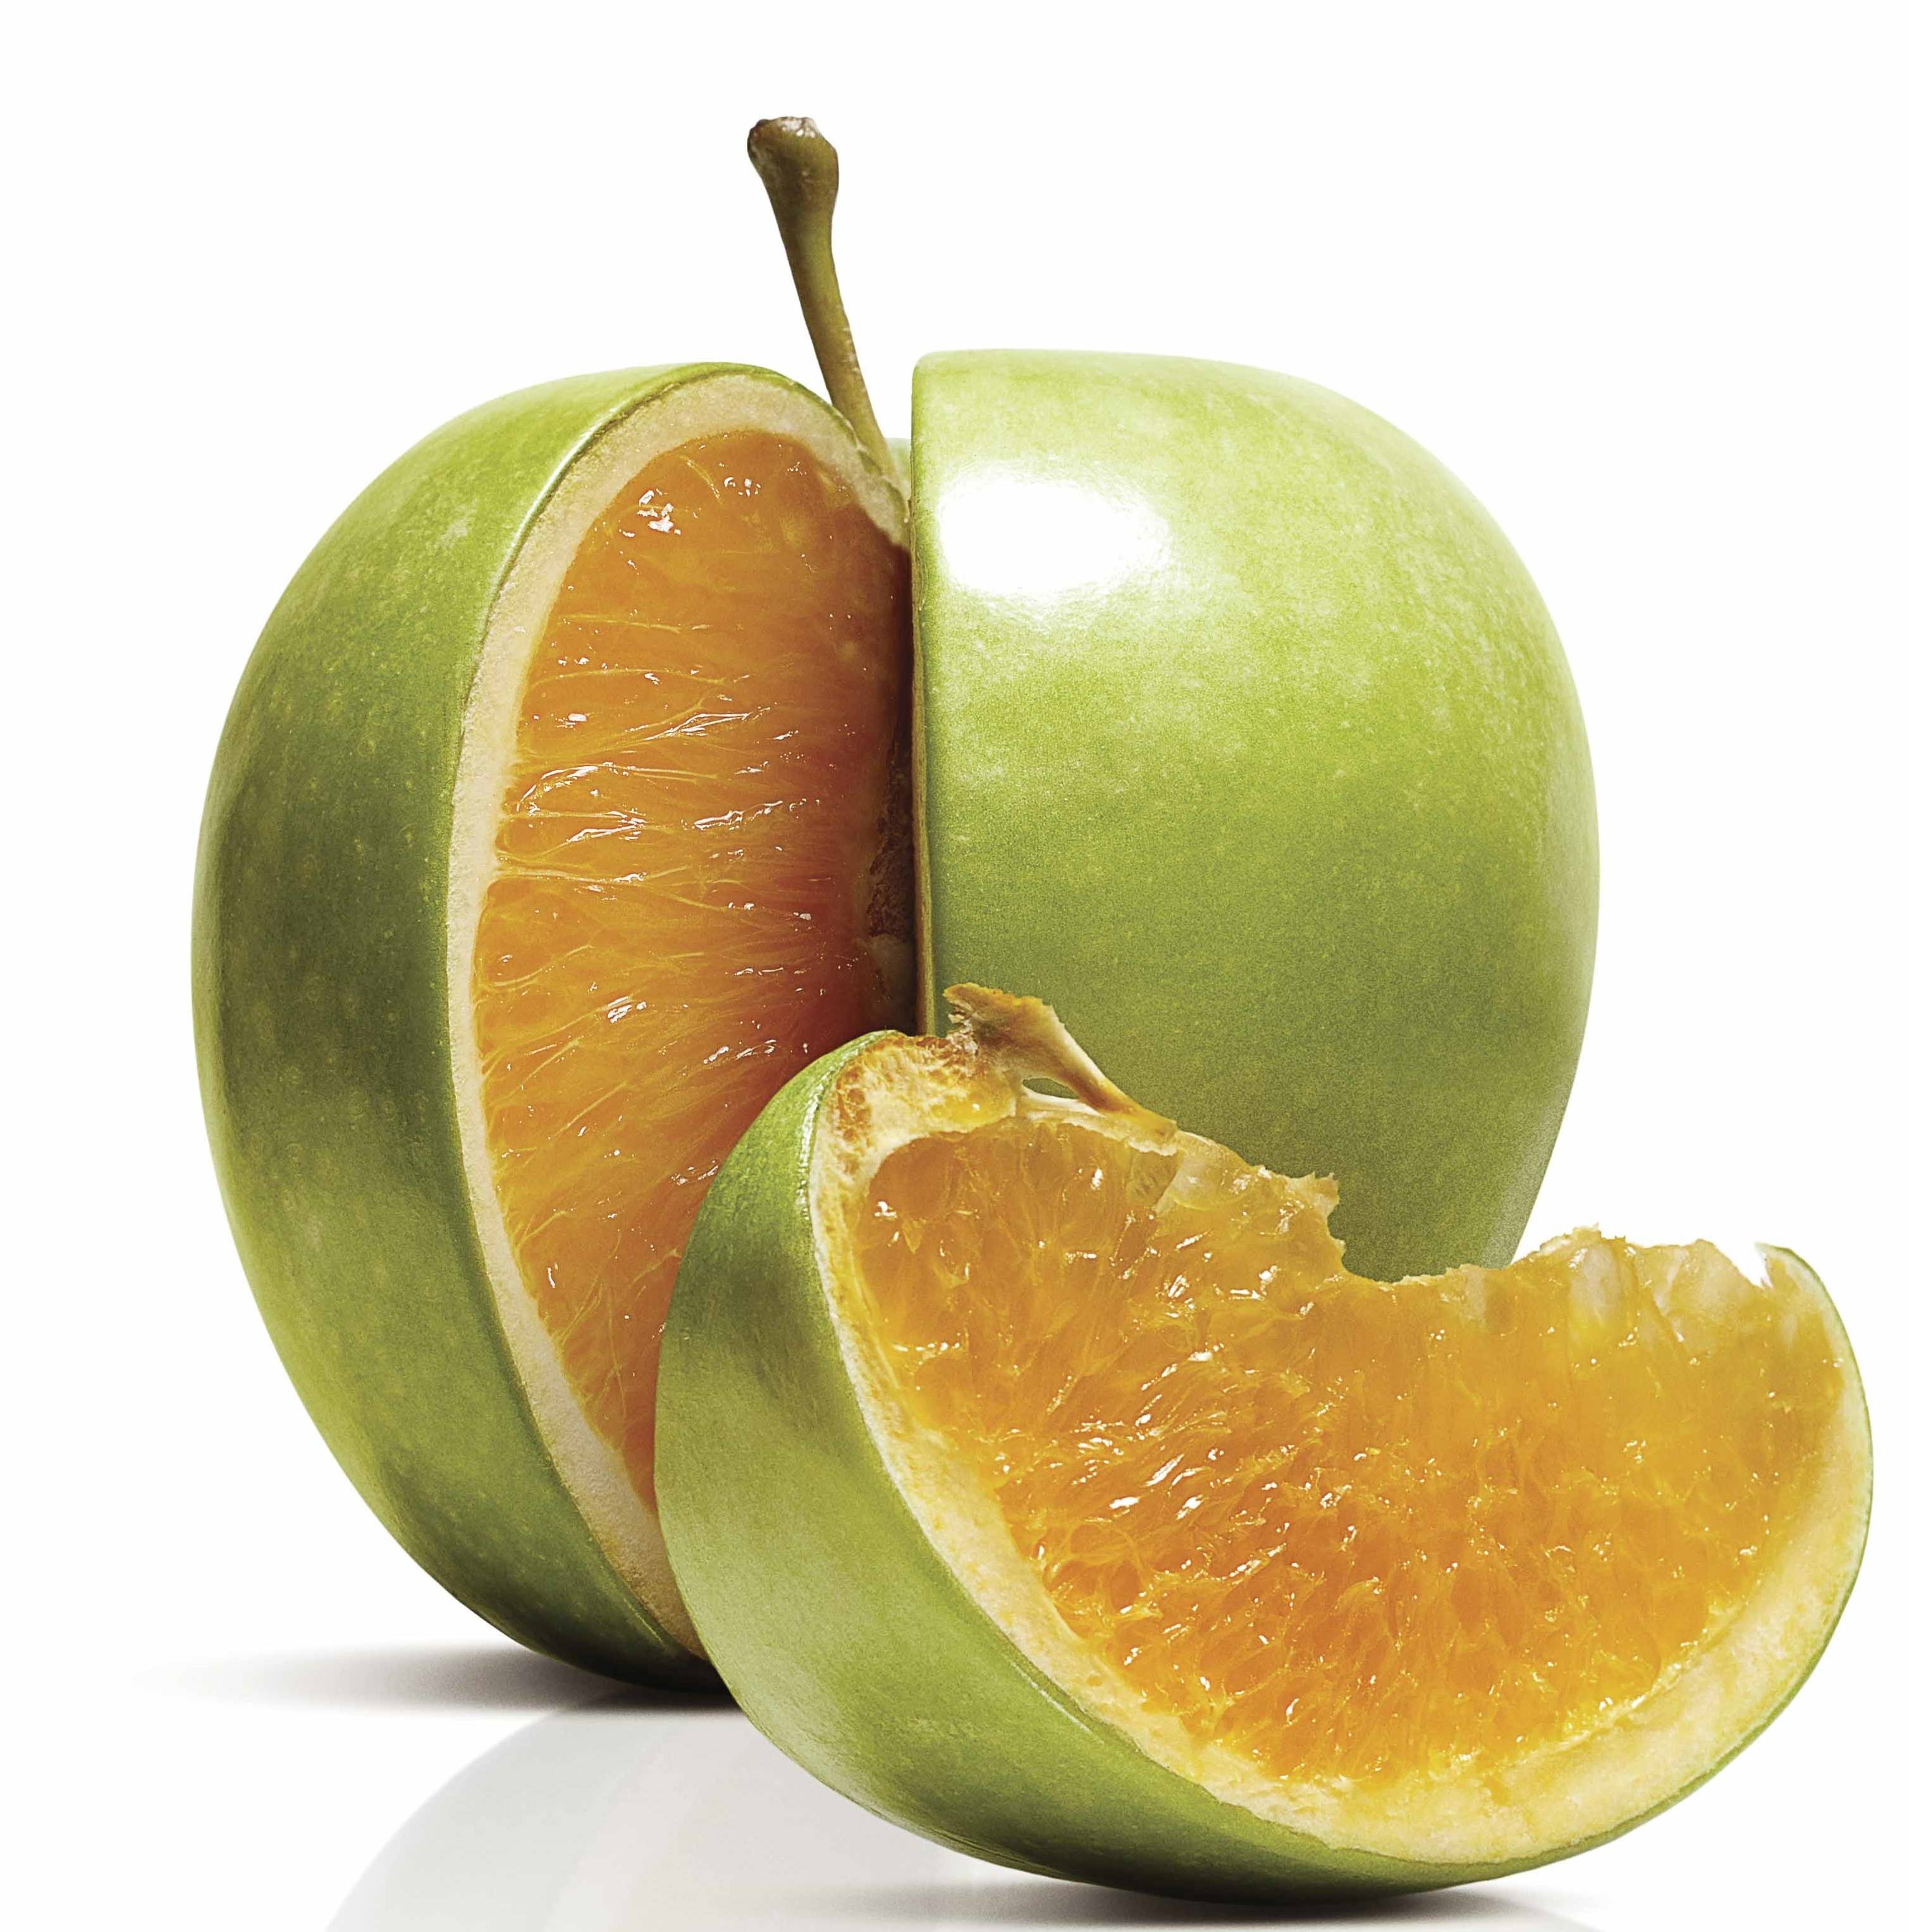
\includegraphics[width=2in]{../graphs/apple-orange}

\column{2in}



\vskip .25cm
Donahoe and Levitt (DL) argue a controversial thesis:

\vskip .1cm{\nv
\hfill easier access to abortion \\\hfill{\it causes} decreased crime.}

\vskip .25cm Proposed mechanism holds that birth is  postponed until the
mother is more ready.

\end{columns}

\sk
{They assume stable family $\Rightarrow$ better upbringing $\Rightarrow$ less crime.}

\vskip .5cm
There's obviously no experiment here.  \\How have they controlled for confounders?

\end{frame}

\begin{frame}[fragile]
{Crime $\sim$ Abortion regression}

{The treatment variable $d$ is by-state abortion rate, \\
and for response we look at {\theme $y=$ murder rate}.}

\vskip .25cm
DL {\it control} for bunch of state-specific {\it confounders}: income, poverty, child tax credits, weapons laws, beer consumption... 

\vskip .2cm
They also include state effects {\gr (factor `$s$')} and a time trend {\gr (numeric `$t$'')} to control for missed confounders.

{\nv \footnotesize
\begin{semiverbatim}
> orig = glm(y ~ d + t + s + ., data=controls) 
> summary(orig)\$coef[`d',]\bk
     Estimate    Std. Error       t value      Pr(>|t|) 
-2.098119e-01  4.109177e-02 -5.105936e+00  4.505925e-07 
\end{semiverbatim}}

{\theme Abortion has a very significant effect!}
Skeptical?  You should be.
\end{frame}



\begin{frame}
{Alternative story: \theme Cellphones and Murder}

{Technology has contributed to
lower murder rates, and we'll add cellphone
subscribers as a variable to control for tech progress.}

\vskip .1cm

{\gr   e.g., Cellphones lead to faster 
ambulances, our jobs are  gentile so we're 
less rough, more communication increases empathy, 
or we don't interact in-person
because we don't have to.}

\vskip .25cm
~~~~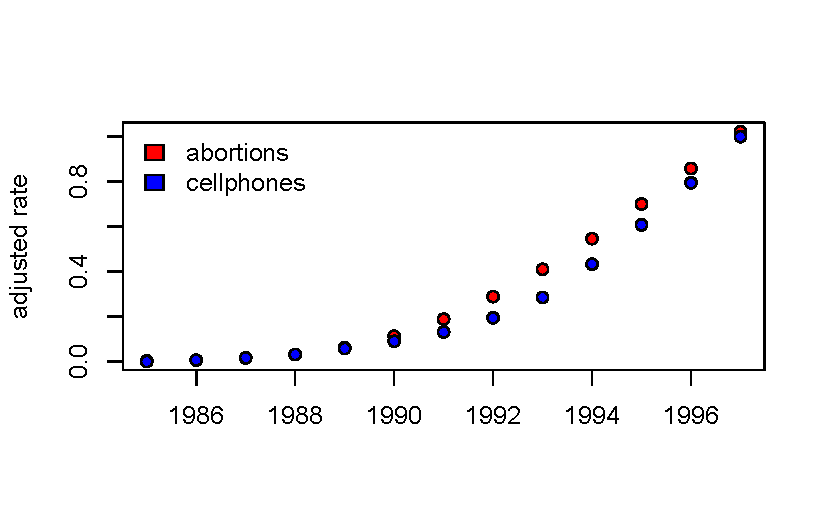
\includegraphics[width=3.75in]{../graphs/cellphone_abortions}

Abortion and cellphones move together...

\vskip -.4cm
\end{frame}

\begin{frame}[fragile]

{\nv \footnotesize
\begin{semiverbatim}
> tech = glm(y ~ phone + t + s + ., data=controls)
> summary(tech)\$coef[c(`phone'),]\bk
     Estimate    Std. Error       t value      Pr(>|t|) 
-3.662545e-01  6.779352e-02 -5.402500e+00  9.699480e-08 
\end{semiverbatim}}

\vskip -.25cm
{\theme \hfill Cellphones have an even more significant effect!}


\sk
It took me about 10 minutes to dream up a\\ causal variable and grab data off of wikipedia.  

\sk What is happening is that murder decreased quadratically,\\
and we have no controls that also moved this way.

\sk
How can we be sure the abortion effect is not just a stand-in
for another cause that changed quadratically over the years?\\


\end{frame}


\begin{frame}[fragile]

To {\it control} for such confounders, we just add {\theme $t^2$} to the model.

\vskip .2cm
We should also allow confounder effects to interact with each other
(e.g., different {\tt gun} effect for high {\tt beer}) and with time.

{\nv \footnotesize
\begin{semiverbatim}
> interact <- glm(y ~ d + (s + .^2)*(t+t2), data=cntrls)
> summary(interact))\$coef['d',]
\bk  Estimate Std. Error    t value   Pr(>|t|) 
 0.8261849  0.7367764  1.1213508  0.2629207 
\end{semiverbatim}}
{\theme Significance disappears.}

\vskip .25cm
This happens because we've added so many variables \\that there is not enough data to say anything is significant.

{\nv \footnotesize\vspace{-.25cm}
\begin{semiverbatim}
> dim(model.matrix(y ~ d + (s + .^2)*(t+t2), data=cntrls))
\bk [1] 624 280
\end{semiverbatim}}


The authors can't be expected to fully control for every crazy story.

\vskip -.5cm
\end{frame}


\begin{frame}
{Multicollinearity and the lasso}

{ MLE treatment effect estimation fails if you have too many controls.} {\it But can't we just throw everything in a lasso?}

\vskip .2cm
Not exactly.  

\vskip .2cm
Even if all possible influencers are in $\bm{x}$, the lasso won't always choose the right ones to remove confounding effects.

\vskip .5cm
In our earlier treatment effect equations, we could have also \\written $\bm{x} = \bs{\varphi}d + \upsilon$, so that $\bm{x}$ is now a function of $d$.
\begin{align*}
\text{Then:~~~~}~\ds{E}[y|\bm{x},d] & = d\gamma + \bm{x}'\bs{\beta} =  d(\gamma + \bs{\varphi}'\bs{\beta}) + \upsilon \bs{\beta}
\end{align*}
Since the lasso makes you pay a price for every extra nonzero coefficient, it'll choose to just collapse the effects of $\bm{x}$  ($\bs{\beta}$) into $\hat\gamma$ \\
{\theme unless $\upsilon$ has a big enough effect to warrant the extra cost.}

\end{frame}

\begin{frame}[fragile]
{Re-visit Hockey}


To guarentee that confounding effects are removed from $\gamma$, \\you need to include them  
in the model {\it without penalty}.


\vskip .2cm
In the hockey homework example, we did exactly this for team-season and skater configuration effects.

\vskip .2cm
This removes, say, time, market, or short-handed effects on performance from our estimates of player performance.

\vskip .5cm
But we then just estimated a lasso path for individual players.

\vskip .2cm
For two players who are always on the ice together, lasso will combine them into a  single (confounded) player effect.

\vskip .2cm
Luckily, there's enough variation here even to separate twins
\begin{semiverbatim}\small\nv\vspace{-.1cm}
      DANIEL_SEDIN HENRIK_SEDIN 
          0.313971     0.257994 
\end{semiverbatim}
\vskip -.5cm
\end{frame}


\begin{frame}
{Treatment Effects with High Dimensional Controls}

We want to use our model selection tools to help estimate\\ $\gamma$ in 
$\ds{E}[y|\bm{x},d] = d\gamma + \bm{x}'\bs{\beta}$ when $\bm{x}$ is high dimensional.

\vskip .1cm
~~~But we need to avoid confusing $\hat\gamma$ with $\bs{\beta}$.


\vskip .5cm

We need to do variable selection in a way that \\still allows us to control for confounding variables.

\vskip .5cm
It is all about prediction: we want to forecast $y$ for new \\random $\bm{x}$ but where {\it $d$ changes independently from $\bm{x}$}.

\end{frame}

\begin{frame}
{Causal Lasso}

We have $d = d(\bm{x}) + \nu$, and {\nv  we want the effect of $\nu$}.

\vskip .1cm
{So estimate $\hat d(\bm{x})$ directly and include it in the regression!}

\vskip .5cm
Any left over effect of $d$ will be attributable to $d-\hat d(\bm{x}) = \nu$.
\[
\ds{E}[y|\bm{x}] = {\theme (\hat d(\bm{x}) + \nu)\gamma} + \hat d(\bm{x})\delta +
\bm{x}'\bs{\beta} = {\theme \nu\gamma} + \hat d(\bm{x})(\gamma+\delta) +
\bm{x}'\bs{\beta}
\]


Controlling for $\hat d(\bm{x})$ in regression is equivalent\\ to estimating $\hat\gamma$ as the effect of $\nu$: {\it the independent part of $d$}. 

\end{frame}


\begin{frame}
{A Treatment Effects Lasso}

Two stages:
\begin{enumerate}
\item Estimate $\hat d(\bm{x})$ with lasso regression of $d$ on $\bm{x}$.
\item Do a lasso of $y$ on [$d$, $\hat d(\bm{x})$, $\bm{x}$], with $\hat d(\bm{x})$ {\it unpenalized}.
\end{enumerate}

\vskip .25cm
Including $\hat d$ unpenalized in [2] ensures that  confounder effects on $d$ have been removed: thus $\hat\gamma$ measures the effect of $\nu$.

\vskip .25cm
In [2], we can apply our usual AICc lasso to see \\what else in $\bm{x}$ effects $y$ and, most importantly, if $\hat\gamma \neq 0$.

\vskip .25cm
We've replaced causal estimation with two prediction problems.

And prediction is something we're really good at, even in HD.


\vskip .25cm
{\theme In the end, we're asking: is $\nu$ {\it useful} for predicting $y$?}

\end{frame}

\begin{frame}[fragile]
{Back to abortion}

{If you just run a straight lasso onto $d$ and $\bm{x}$,\\
AICc selects a significant negative abortion effect.}

\begin{semiverbatim}\nv
> naive <- gamlr(cBind(d,x),y)
> coef(naive)["d",]\bk
[1] -0.09005649
\end{semiverbatim}

\end{frame}

\begin{frame}[fragile]


{But AICc lasso selects $d$ as highly predicted by $\bm{x}$.}

\vskip .25cm
{\nv \tt treat <- gamlr(x,d,lambda.min.ratio=1e-4)\\
dhat <- predict(treat, x, type="response") }
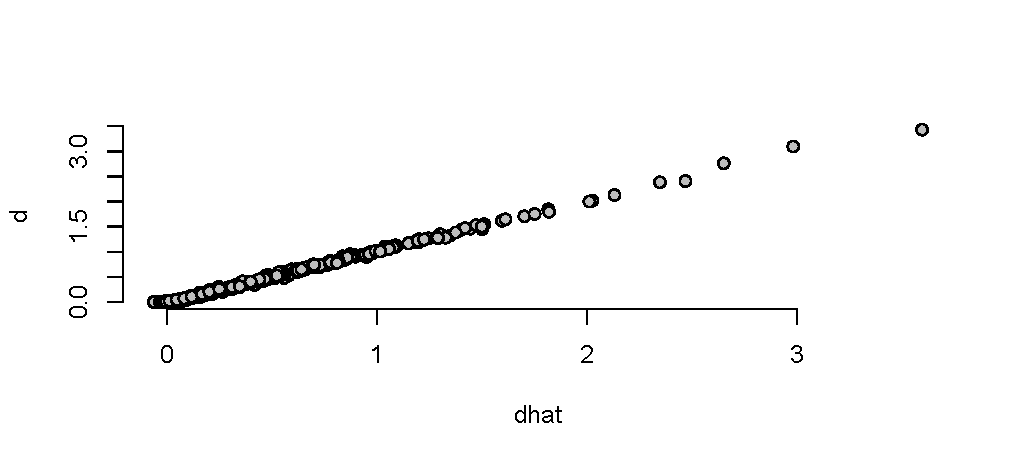
\includegraphics[width=4.25in]{AbortionDhat}

In Sample $R^2$ is $>$99\%.

\vskip .1cm
So there's almost no {\it independent} movement of abortion rates to measure as effecting crime (it's not much of an experiment).

\end{frame}

\begin{frame}[fragile]

{Sure enough, if you include {\tt dhat} in lasso regression \\then AICc says there is no residual effect for $d$.}

\begin{semiverbatim}\gr
## free=2 here leaves dhat unpenalized\nv
> causal <- gamlr(cBind(d,dhat,x),y,free=2)
> coef(causal)["d",] \bk
[1] 0
\end{semiverbatim}

Summary: causation via two prediction models.
\begin{itemize}
\item Fit $\hat d$: your best predictor for $d$ from $\bm{x}$.
\item Find the best predictor for $y$ from $d$ and $\bm{x}$, \\after influence of $\hat d$ is removed {\gr (i.e., predict $y$ from $\nu$ and $\bm{x}$)}.
\end{itemize}
Then $\hat \gamma$ predicts what will happen if we change $d$ independently.

\end{frame}

% \begin{frame}
% {BCH algorithm}

% Belloni + Chernozhukov + Hansen have a related algorithm:
% \begin{itemize}
% \item do lasso regression for $y \sim \bm{x}$, and for $d\sim \bm{x}$.\\
% {\gr You can use, e.g., AICc selection for each lasso path.}
% \item say
%  variables  with nonzero effects in {\it either} model are {\tt controls}, and 
%  fit MLE {\tt glm(y $\sim$ d + controls)}.
% \end{itemize}
% {The {\tt glm} p-value for $d$ is then your treatment-effect significance.}

% \sk
% This algorithm is similar to ours, 
% and the intuition is the same.

% However, the selected {\tt controls}  are unpenalized in {\tt glm}.

% \vskip .2cm\nv
% The upshot is that, with a lot of very tough math, they show you  interpret the $p$-value as usual: we can do frequentist inference!
% \end{frame}

% \begin{frame}[fragile]
% {BCH on Abortion}

% \vskip .25cm
% First, do 2 lasso regressions to get controls (chooses $\approx 300$).
% \begin{semiverbatim}\small\nv
% donx <- gamlr(x,d)
% dpreds <- which(coef(donx)[-1]!=0)
% yonx <- gamlr(x,y)
% ypreds <- which(coef(yonx)[-1]!=0)
% inthemmodel <- unique(c(dpreds,ypreds))
% \end{semiverbatim}

% \vskip .25cm
% Second, run an MLE linear regression and look at significance.
% \begin{semiverbatim}\nv\small
% causal_glm <- glm(y~d+., data=x[,inthemodel])
% summary(causal_glm)\$coef["d",] \bk
%   Estimate Std. Error    t value   Pr(>|t|) 
% -0.3163973  0.3703234 -0.8543811  0.3935174 
% \end{semiverbatim}

% {BCH agree: \it no significant independent effect of abortion.}
% \end{frame}

% \begin{frame}
% {Frequentist Inference}

% Estimating $\hat d$ and using it as a control is explicitly  predictive: \\select the best predictor when $d$ changes independent from $\bm{x}$.

% \vskip .5cm
% BCH use the same `double prediction' logic:\\ 
% \hskip 3cm {\nv include $x_j$ that predict $d$ {\it or} $y$.}\\
%   But they then work very hard to find a procedure that\\ preserves the usual standard error calculations for $\gamma$.

% \vskip .1cm{\gr
% This is non-trivial.  They're mimicking the low-D controls setting, even though $\bm{x}$ has actually been selected from an HD set.}

% \sk{\theme 
% Accurate standard errors are \it essential for  frequentist inference.}  

% % \vskip .2cm
% % For those of us better at algorithms then asymptotics, \\there's another option.

% \end{frame}


\begin{frame}
{Observational Study Wrap-Up}

Science is hard.  Keep theorizing, but hit ideas with data.

\vskip .1cm
We can't say that abortion {\it does not} lower crime. \\We just have nothing that looks like an experiment here.

\vskip .1cm
And an experiment (or something that looks like one) \\is what you need to estimate TEs.


\vskip .5cm
Our double-lasso  is one [good] way to sort out causation.

But this is a huge area, and there are {\it many} strategies: {\gr matching, instrumental variables, double robust, post lasso...}

\vskip .5cm
Always ask yourself:
\begin{itemize}
\item How well would my model predict if I change $d$ arbitrarily?
\item How am I replicating what I'd get from a real experiment?
\end{itemize}

\end{frame}

\begin{frame}
{Frequentist Uncertainty}

Switching gears: {\nv wait, what is your uncertainty about $\hat \gamma$?}

\vskip .5cm
This class has paid little attention to {\it standard errors}.\\
{In other stats classes, SEs are often a main focus.}

\vskip .5cm
This isn't because we don't care, but because
the theoretical SEs you've learned elsewhere are incorrect for 
Big Data:
\begin{itemize}
\item They don't account for model selection
\item They only apply independently.
\end{itemize}

\vskip .25cm
Instead, we'll use a {\it non parametric} method: the bootstrap.


\end{frame}

\begin{frame}

\vskip .25cm
Recall your early stats: {\theme the sampling distribution.}

\vskip .1cm
Imagine getting multiple datasets of size $n$ from the population.

\vskip .1cm
The {\it sampling distribution} of an estimator $\hat \beta$\\ is
the histogram of your estimates for each dataset.


\vskip .25cm
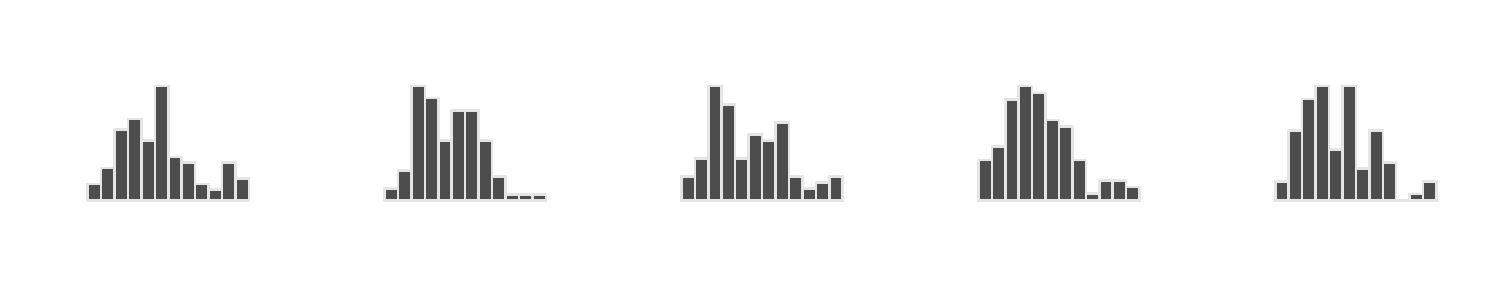
\includegraphics[width=4.2in]{../graphs/bs_boothist}

\vskip -.2cm
$
~\begin{array}{c}\downarrow\\
	\hat\beta_1\\
	~~\searrow
\end{array}
$
\hskip 1.1cm
$
\begin{array}{c}\downarrow\\
	\hat\beta_2\\
	~~\searrow
\end{array}
$
\hskip 1.1cm
$
\begin{array}{c}\downarrow\\
	\hat\beta_3\\
	\downarrow
\end{array}
$
\hskip 1.1cm
$
\begin{array}{c}\downarrow\\
	\hat\beta_4\\
	\swarrow~~
\end{array}
$
\hskip 1.1cm
$
\begin{array}{c}\downarrow\\
	\hat\beta_5\\
	\swarrow~~
\end{array}
$

\begin{center}
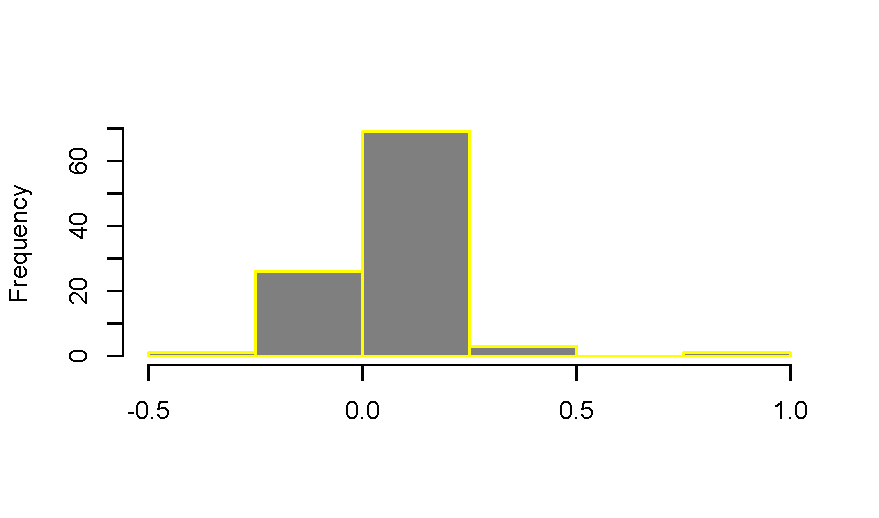
\includegraphics[width=2.25in]{boothist}
\end{center}


\vskip -.5cm
\end{frame}

\begin{frame}


{\bf \theme The Bootstrap:} resample your data {\it with replacement} \\
~~~~~~~~~~~~~~~~~~ and calculate  some statistic of interest.  

\vskip .1cm {\it \gr With-Replacement: each draw is put back in the `bucket', so it is possible to sample the same
observation multiple times.  }

\sk
To raise oneself up by bootstraps...  
{\gr (Try it; it doesn't work).}

\vskip .05cm    The metaphor refers
to surprising examples of self sufficiency.

\vskip .5cm
For $b=1\ldots B$ `bootstrap samples'
\begin{itemize}\nv
\item Resample {\theme with replacement} $n$ observations.
\item Calculate your estimate (e.g., $\hat\beta_b$).
\end{itemize}

\sk
This is an {\it approximation} to the sampling distribution.

\vskip .1cm
For example, an approx SE($\hat\beta$) is
$\mr{sd}(\hat\beta) =\sqrt{\frac{1}{B}
\sum_b (\hat \beta_b - \bar{\beta})^2}.
$

\end{frame}


\begin{frame}[fragile]
{\large A simple bootstrap}

\begin{semiverbatim}\footnotesize
data(airquality); laq <- log(airquality[,1:4])
mle <- glm(Ozone \til Solar.R+Wind+Temp, data=laq)

\vspace{-.6cm}{\nv
gamma <- c(); n <- nrow(airquality)
for(b in 1:100)\{
   ib <- sample(1:n,n,replace=TRUE)
   fb <- glm(Ozone \til Solar.R+Wind+Temp, data=laq, subset=ib)
   gamma <- c(gamma,coef(fb)["Temp"]) \}}

\vspace{-.6cm}
hist(gamma); abline(v=coef(mle)["Temp"], col=2)
\end{semiverbatim}

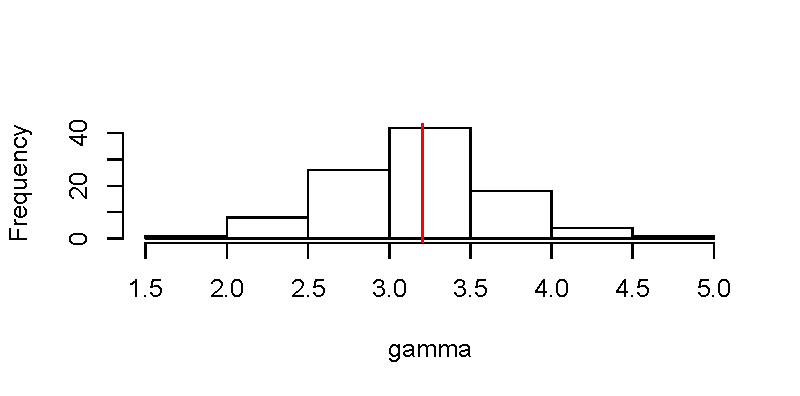
\includegraphics[width=\textwidth]{AirQualBoot}
\vskip -.25cm
\end{frame}

\begin{frame}

{\bf \theme The Bootstrap: \bk why it works}

\begin{center}
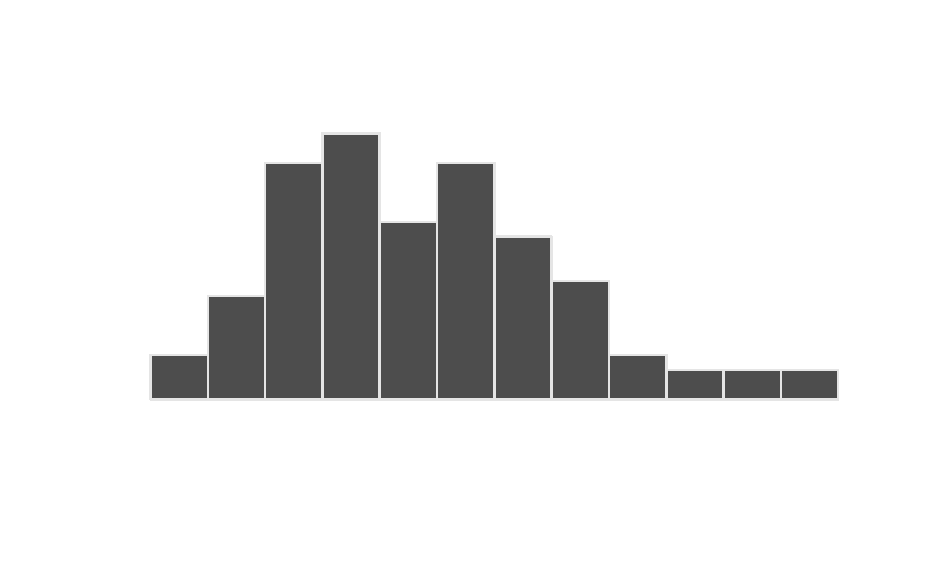
\includegraphics[width=2in]{../graphs/bs_bighist}

{\gr data sample}

$\swarrow~~~\downarrow~~~\searrow$

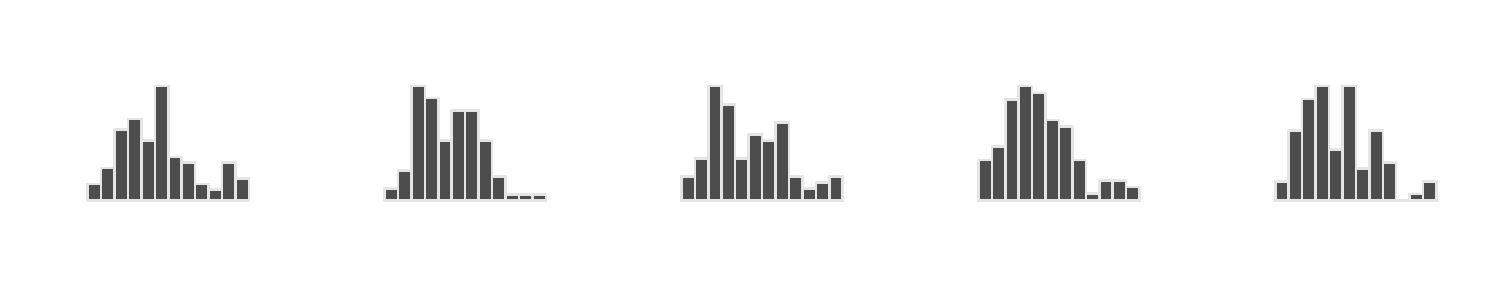
\includegraphics[width=4.25in]{../graphs/bs_boothist}

\gr bootstrap samples
\end{center}

You are pretending that the {\it empirical data distribution} is
the population, and using it to draw alternative samples.
\end{frame}



% \begin{frame}
% {Bootstrap and Cross Validation}


% We're  using the variation you notice in CV to our advantage.

% {The difference between Boots and CV is `with' replacement.}


% \sk
%  CV is great for understanding OOS prediction.\\
% For sampling distributions, it  underestimates
% uncertainty.

% \vskip .1cm
% This is because the resample is forced to look like your sample.\\
% {\gr Think of $n$-fold (or leave-one-out) to convince yourself.}

% \sk  On the other hand, you  underestimate predictive uncertainty by 
% re-calculating   residuals $\{e_1 \ldots e_n\}$ for each bootstrap model fit.

% \vskip .1cm
% This is because fit includes $\varepsilon_i$, the unpredictable part of each
% observation, for those in the bootstrap sample.  

% \end{frame}



\begin{frame}
{Conditional vs Unconditional SE}

Bootstraps and {\tt glm} $p$-values measure different things:
 
 \vskip .1cm
 {\nv Bootstraps see how $\hat \beta$ varies for random draws from the {\it joint} distribution for $[\bm{x},y]$. } {\color{DarkGreen} MLE standard errors measure variation \\in 
 $\hat \beta$ for random draws from the {\it conditional} distribution $[y|\bm{x}]$.
}

\sk
Bootstrap uncertainty is more appropriate if you have an observational study: $\bm{x}$ was random (e.g., abortion).  

\vskip .1cm
MLE errors are appropriate for a designed experiment: \\you picked $\bm{x}$ (e.g., paid search).

\sk
You can also build bootstraps for conditional SEs, \\using parametric and semiparametric bootstraps.
\end{frame}

\begin{frame}


If we go back to our air quality data, we can compare the theoretical 95\% CI to the bootstrapped sampling distribution.

\sk
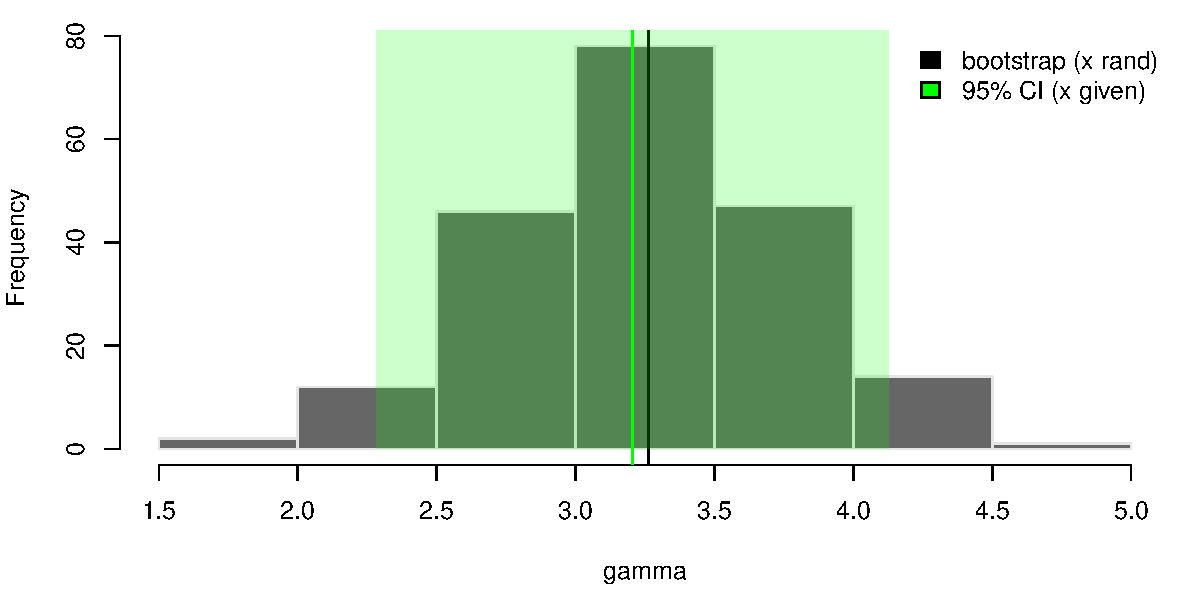
\includegraphics[width=\textwidth]{airboot}

\vskip .1cm
Centered in the same place, but bootstrap uncertainty is wider.

\end{frame}


\begin{frame}[fragile]

{We can also bootstrap the double lasso TE estimator.}

\vskip .1cm
For each bootstrap data resample,
\begin{itemize}
\item re-fit regression $d\sim \bm{x}$ to get $\hat d (\bm{x})$.
\item re-fit $y \sim [d,\hat d(\bm{x}),\bm{x}]$ with $\hat d$ unpenalized ({\tt free}).
\item store $\hat \gamma$, the coefficient on $d$.
\end{itemize}

\vskip .25cm
For abortion, we get a boring answer:
\begin{semiverbatim}\nv\small
> summary(gamma\_boots) 
   Min. 1st Qu. Median Mean 3rd Qu. Max. 
      0       0      0    0       0    0 
\end{semiverbatim}
Sampling distribution for AICc selected $\hat \gamma$ is a point at zero.

{\gr i.e., we imagine that given another random sample from the data population we'd make the same conclusion nearly always.}


\end{frame}



% \begin{frame}
% {Bootstrapping Abortion: BCH routine}

% $\hat\gamma$ doesn't get set to zero, so we have more to look at.


% \vskip .25cm
% 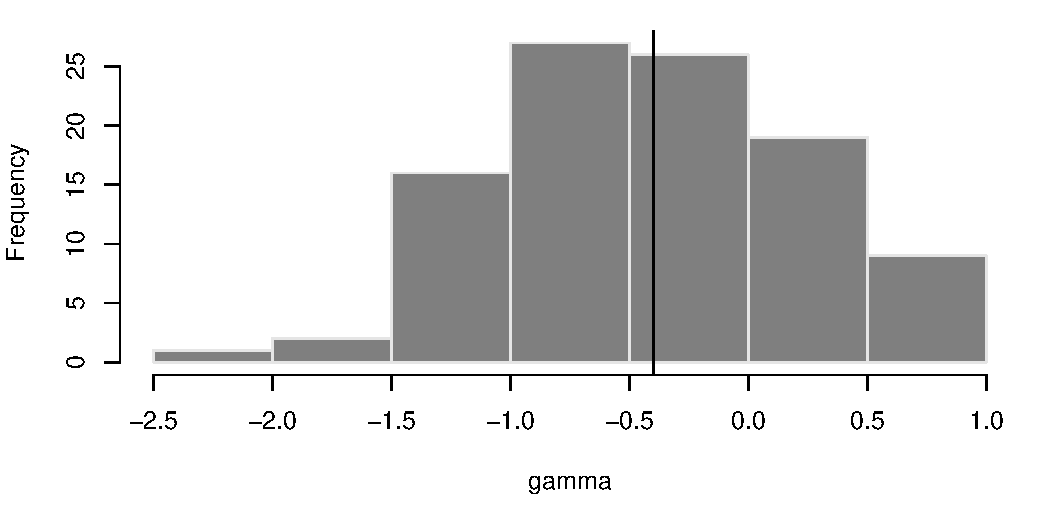
\includegraphics[width=\textwidth]{abortion_boothist}


% About 2/3 of the sampling distribution is below zero here.

% {\gr Your run may include some really big $\hat\gamma_n$: MLEs are unstable!.}

% \end{frame}

\begin{frame}
{\theme The Bootstrap: \bk when it doesn't work}

\vskip .25cm
Basically, when the empirical data distribution (EDF)\\
is a poor substitute for the population distribution.

\vskip .1cm
{\it There's also plenty of settings where it `works', \\but the uncertainty target is not what you'd expect.}

\sk
{\nv Dimension matters}

\vskip .1cm
This happens when your sample is small, or  
when \\the statistic you want to bootstrap is high dimensional.

\vskip .25cm
When it breaks, the bootstrap underestimates uncertainty:\\
You haven't seen enough data to have variability in the EDF.

{\gr In such settings, theoretical SEs are also usually useless.}

\vskip .25cm
As a rule: you can bootstrap a low dimensional statistic.

\end{frame}


\begin{frame}
{Homework: Networks and Microfinance}

{Banerjee, Chandrasekhar, Duflo, Jackson 2012: \\
social networks in india and microfinance adoption.}

\vskip .5cm
They have info about households in a collection of rural
villages, and data on whether each household made use of
 micro-finance facilities when they were made available.

 \vskip .1cm
 There is economic/anthropological/sociological interest in 
 what cultural practices lead to adoption of commercial lending.

\vskip .5cm
In particular, they ask whether being more `connected' \\makes you more or less likely to engage in microfinance.

{\gr `network effects' are very trendy in bio and econ.}

\end{frame}

\begin{frame}
{Network Degree}

They surveyed households in  rural indian villages about friendships, business partnerships, and religious ties.  

\vskip .25cm
I've coded this in {\tt microfi\_edges} as a zero/one connection.

The {\it edges} between household {\it nodes} define networks.

\vskip .25cm
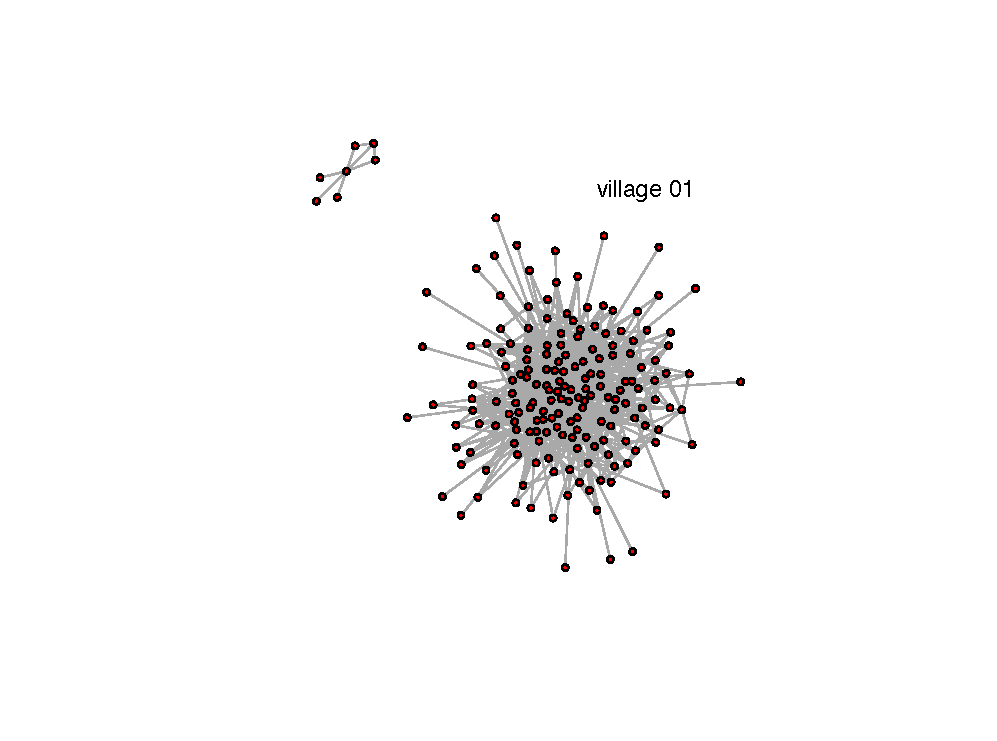
\includegraphics[width=2in]{microfi_village01}
~~
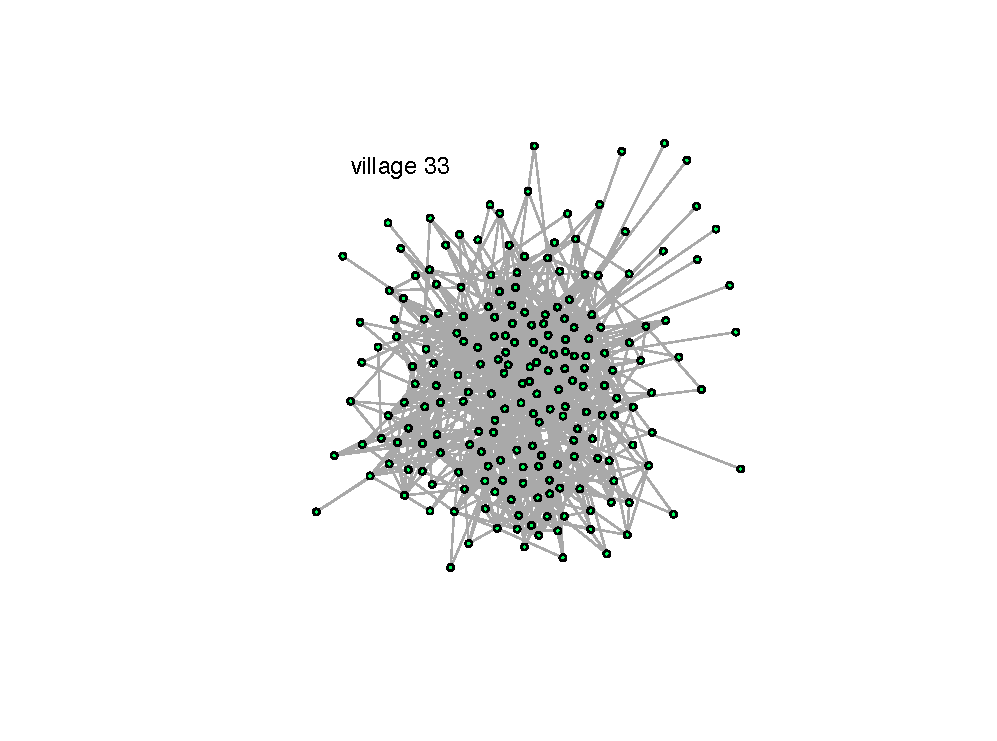
\includegraphics[width=2in]{microfi_village33}

\vskip -.25cm
~~village 01~~~~~~~~~~~~~~~~~~~~~~~~~~~~~~~ village 33
\vskip -.5cm

\end{frame}

\begin{frame}

A summary of node connectivity is its degree:
its edge count.  

{\gr This is the number of `relationships'  that a household has.}

\vskip .25cm
We'll ask a version of the question in the paper: 

\vskip .1cm
{\nv ~~~~~~~Is this connectivity structurally connected \\
~~~~~~~to propensity to get a microfinance loan?}

\vskip .1cm
{\gr Are well connected household more likely to seek a loan \\(because they are comfortable with outside finance)?

\vskip .1cm

Or are they less likely (because their network provides the support they need already)?

\vskip .1cm
Or, more modestly, are the characteristics that increase connectivity correlated with being amenable to microfinance?}

\vskip .25cm
Plenty of holes to pick, and I've no idea what direction causation goes, but it's at least a fun exploration.

\end{frame}

\begin{frame}
{Homework due next lecture}

\small
[1]. I'd transform {\tt degree} to create our treatment variable $d$. \\ ~~~~~~What would you do and why?

\vskip .1cm
[2].  Build a model to predict $d$ from $\bm{x}$, our controls.\\
~~~~~~Comment on how tight the fit is, and what that \\~~~~~~implies for estimation of a treatment effect.

\vskip .2cm
[3]. Use predictions from [2] in an  estimator for effect of $d$ on {\tt loan}.

\vskip .2cm
[4]. Compare the results from [3] to those from a straight (naive) lasso \\~~~~~~for {\tt loan} on $d$ and $\bm{x}$.  Explain why they are similar or different.

\vskip .2cm
[5]. Bootstrap your estimator from [3] and describe the uncertainty.

\vskip .2cm
[+].  Can you think of how you'd design an experiment\\~~~~~~ to estimate the treatment effect of network degree?

\vskip .5cm
\hfill \gr NB: {\tt loan} is binary.
\end{frame}

\end{document}
